\chapter{Release 2 : Planification Locale et Consolidation Groupe (Sprints 2 et 3)}
\label{chap:sprints_2_3}

\section{Introduction}
Une fois le socle technique et les mécanismes de sécurité validés lors du Sprint 1, l'équipe projet a pu se consacrer au développement du cœur métier de \textit{Cofat Capacity Study}. Cette Release 2, subdivisée en deux Sprints majeurs (Sprint 2 et Sprint 3), constitue la véritable rupture technologique pour les employés du groupe. Dans un premier temps, le Sprint 2 vise à outiller les responsables d'usines (Site Managers) en remplaçant leurs processus manuels par des modules digitaux de planification locale des Équipements, des Espaces et des Ressources Humaines, incluant un algorithme robuste d'importation de fichiers Excel. Dans un second temps, le Sprint 3 exploite l'architecture centralisée de la base de données pour générer, à la volée, les consolidations à l'échelle mondiale (Cofat Group). Ce chapitre aborde enfin la mise en place du référentiel \textit{StandardInvestment V2}, outil décisif pour l'évaluation standardisée des futurs investissements industriels du Groupe COFAT.

\section{Sprint 2 : Déploiement des modules de Planification Locale}
La planification locale est l'action par laquelle chaque usine projette ses besoins capacitaires en fonction des commandes automobiles à venir. L'objectif de ce sprint était de numériser cette étape de manière transparente, en conservant la souplesse d'Excel tout en apportant la rigueur d'une base de données relationnelle.

\subsection{Le Module des Équipements Industriels}
L'objectif du module «~Équipements~» est de permettre au Site Manager de suivre l'état de saturation de son parc de machines (presses, coupeuses, soudeuses) et d'identifier rapidement les goulots d'étranglement qui pourraient bloquer la production d'un nouveau projet automobile.

\vspace{0.5cm}
\begin{figure}[H]
    \centering
    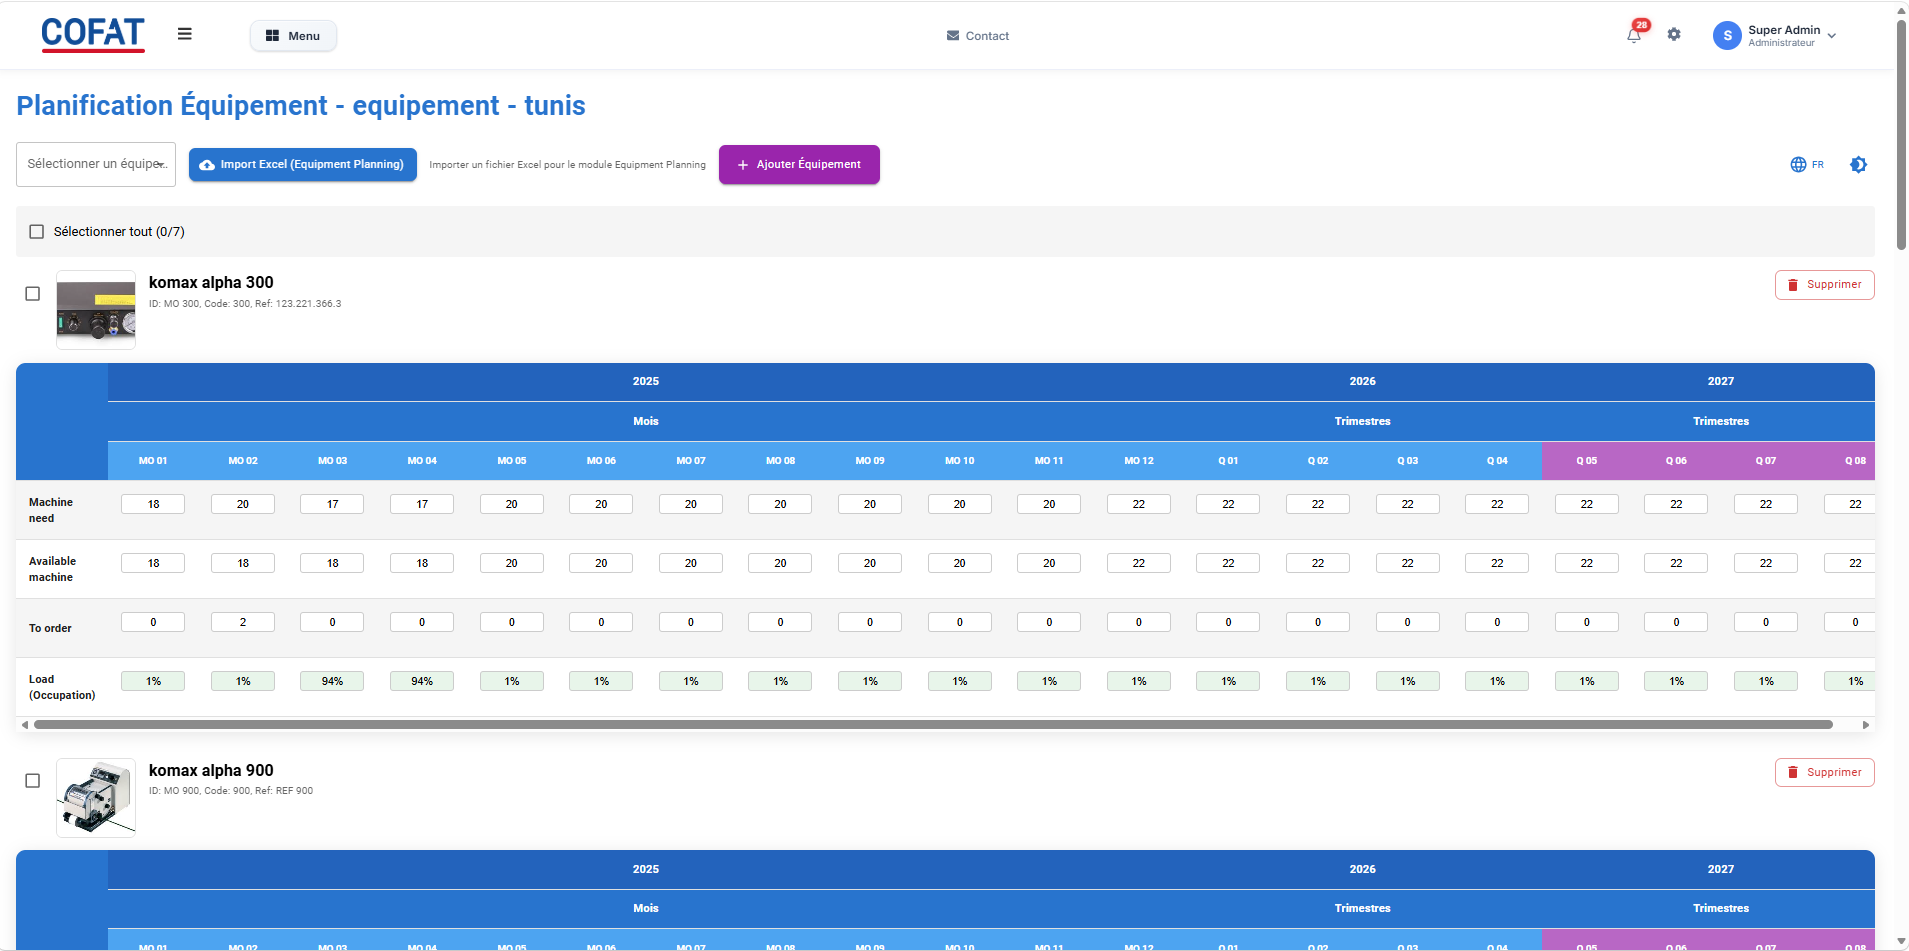
\includegraphics[width=1\textwidth]{img/planification equipement standard.png}
    \caption{Interface de planification locale des équipements industriels}
    \label{fig:planif_equipement}
\end{figure}
\vspace{0.5cm}

\textbf{Analyse détaillée de l'interface (Figure \ref{fig:planif_equipement}) :}
La conception de cette interface a privilégié la clarté visuelle, car l'ingénieur méthodes doit scanner des dizaines de lignes en un clin d'œil. Le tableau de données, implémenté avec la DataGrid de Material UI, présente les colonnes suivantes :
\begin{itemize}
    \item \textbf{Type d'Équipement} : La désignation de la machine (ex: Komax Alpha 530, Schleuniger).
    \item \textbf{Opération} : L'application permet un filtrage dynamique par étape de production. L'utilisateur peut isoler les machines de la zone «~1-COUPE~», «~2-PREPARATION~», «~3-ASSEMBLAGE~» ou «~4-CONTROLE ELECTRIQUE ET CONDITIONNEMENT~».
    \item \textbf{machineNeed} : Le besoin calculé par l'ingénieur méthodes (par exemple 4.5 machines requises pour absorber le volume commandé).
    \item \textbf{availableMachine} : Le parc physique réel sur le site (par exemple 4 machines actives).
    \item \textbf{load (\%)} : C'est le taux de charge, la métrique fondamentale. Il est calculé selon la formule $Load = (machineNeed / availableMachine) \times 100$. Un code couleur visuel alerte immédiatement l'ingénieur :
        \begin{itemize}
            \item \textbf{Vert (Load $\le$ 80\%)} : Sous-charge, l'usine a de la marge disponible.
            \item \textbf{Orange (80\% $<$ Load $\le$ 100\%)} : Zone de tension, l'équipement est optimisé au maximum.
            \item \textbf{Rouge (Load $>$ 100\%)} : Surcharge critique nécessitant une commande immédiate.
        \end{itemize}
    \item \textbf{toOrder} : Ce champ calcule le déficit. Si le load dépasse 100\%, il indique le nombre d'unités manquantes à acquérir.
\end{itemize}

\textbf{Architecture du modèle \texttt{EquipmentPlanning} :}
Ce tableau de données est directement piloté par la table \texttt{EquipmentPlanning} en base SQL Server. Le modèle Sequelize correspondant impose une contrainte d'unicité composite sur les champs \texttt{(siteId, equipmentId, year, month)}, garantissant qu'un site ne peut avoir qu'une seule entrée de planning pour un équipement donné à une période donnée. Cette contrainte évite les doublons qui fausseraient les calculs de charge.

\subsection{Le Module d'analyse de l'Occupation des Espaces}
L'espace physique (surface au sol en m²) est une contrainte dure dans une usine de câblage. Une ligne d'assemblage ne peut pas être superposée avec une autre. Le module «~Espaces~» permet d'avoir une vision cartographiée et quantitative de la surface disponible pour accueillir de futurs projets.

\vspace{0.5cm}
\begin{figure}[H]
    \centering
    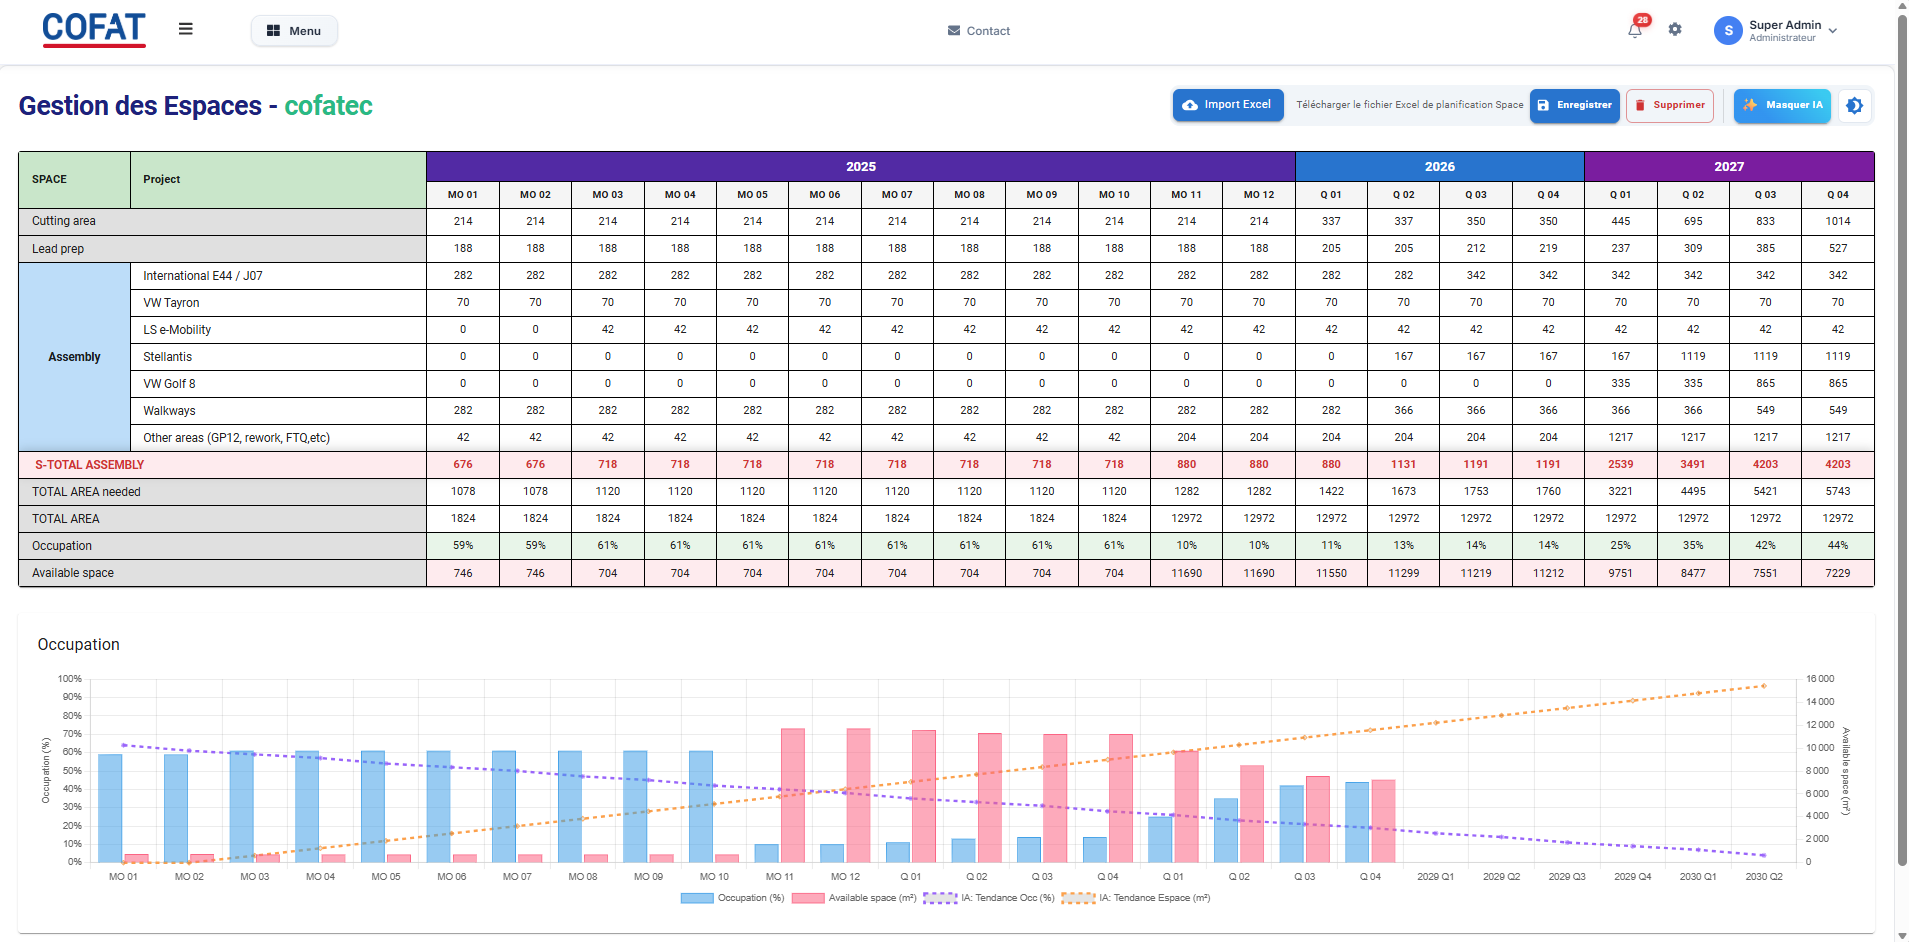
\includegraphics[width=0.9\textwidth]{img/analyse des espaces.png}
    \caption{Tableau de gestion des surfaces par zone de production}
    \label{fig:tableau_espaces}
\end{figure}
\vspace{0.5cm}

\vspace{0.5cm}
\begin{figure}[H]
    \centering
    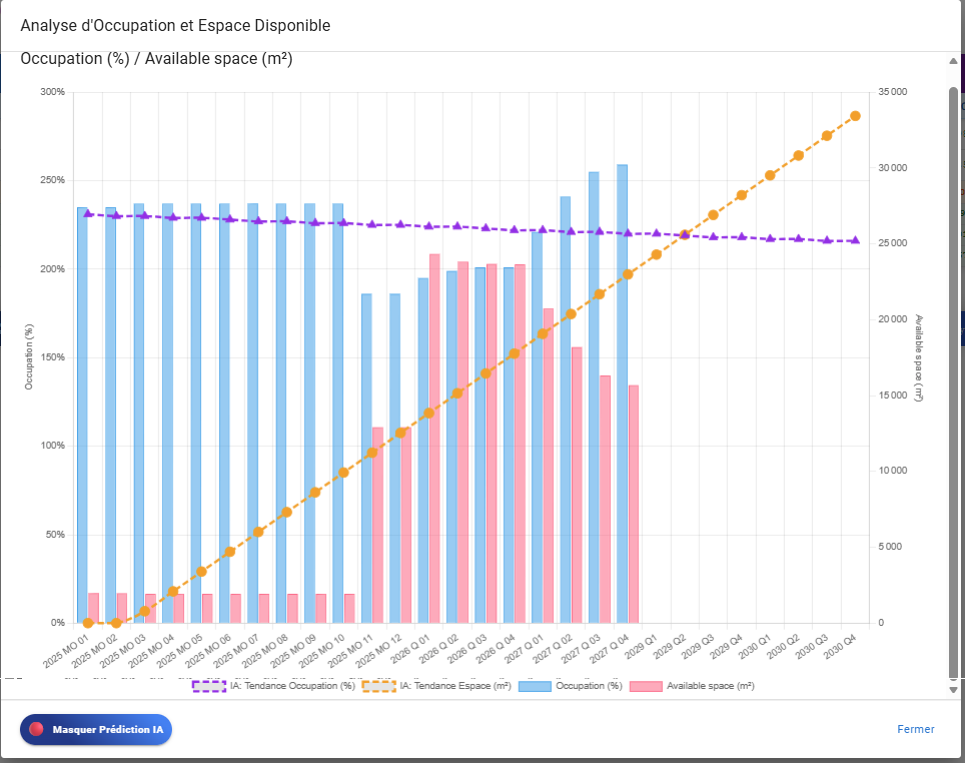
\includegraphics[width=0.9\textwidth]{img/analyse d'occupation et espace disponible.png}
    \caption{Tableau de bord visuel : Taux d'occupation global du site}
    \label{fig:graphique_espaces}
\end{figure}
\vspace{0.5cm}

\textbf{Analyse du fonctionnement du module Espaces :}
Comme illustré dans la Figure \ref{fig:tableau_espaces}, l'interface sépare l'usine en grandes zones logiques. On y retrouve les zones de traitement primaire (\textit{Cutting area}, \textit{Lead prep}) et les vastes halls dédiés aux projets clients majeurs (visibles dans l'interface : \textit{VW Tayron}, \textit{International E44}, \textit{Stellantis J4U}, \textit{VW Golf 8}, \textit{LS e-mobility BEV-A}).

Pour chaque zone, l'ingénieur déclare la surface totale disponible et la surface occupée. Le modèle \texttt{Spaces} en base de données stocke le champ \texttt{area} (surface) ainsi que les informations de typage (\texttt{type}, \texttt{category}) qui permettent de distinguer les zones de coupe, de préparation et d'assemblage.

La Figure \ref{fig:graphique_espaces} met en évidence la puissance de la bibliothèque \textit{Charts.js}. Le composant React extrait les données via l'API et génère un diagramme circulaire (Pie Chart) montrant, d'un coup d'œil, le ratio Espace Occupé / Espace Libre pour l'usine entière. Ce graphique interactif aide le directeur de site à décider rapidement s'il peut accepter la ligne de production d'un nouveau modèle de véhicule ou s'il doit envisager une extension de bâtiment.

\subsection{Le Module de prévision des Ressources Humaines (RH)}
Le recrutement et la formation des opérateurs de câblage prennent des semaines. Le module RH permet d'anticiper les embauches sur un horizon de trois ans, répartis par catégories de personnel et par projets de véhicules automobiles.

\vspace{0.5cm}
\begin{figure}[H]
    \centering
    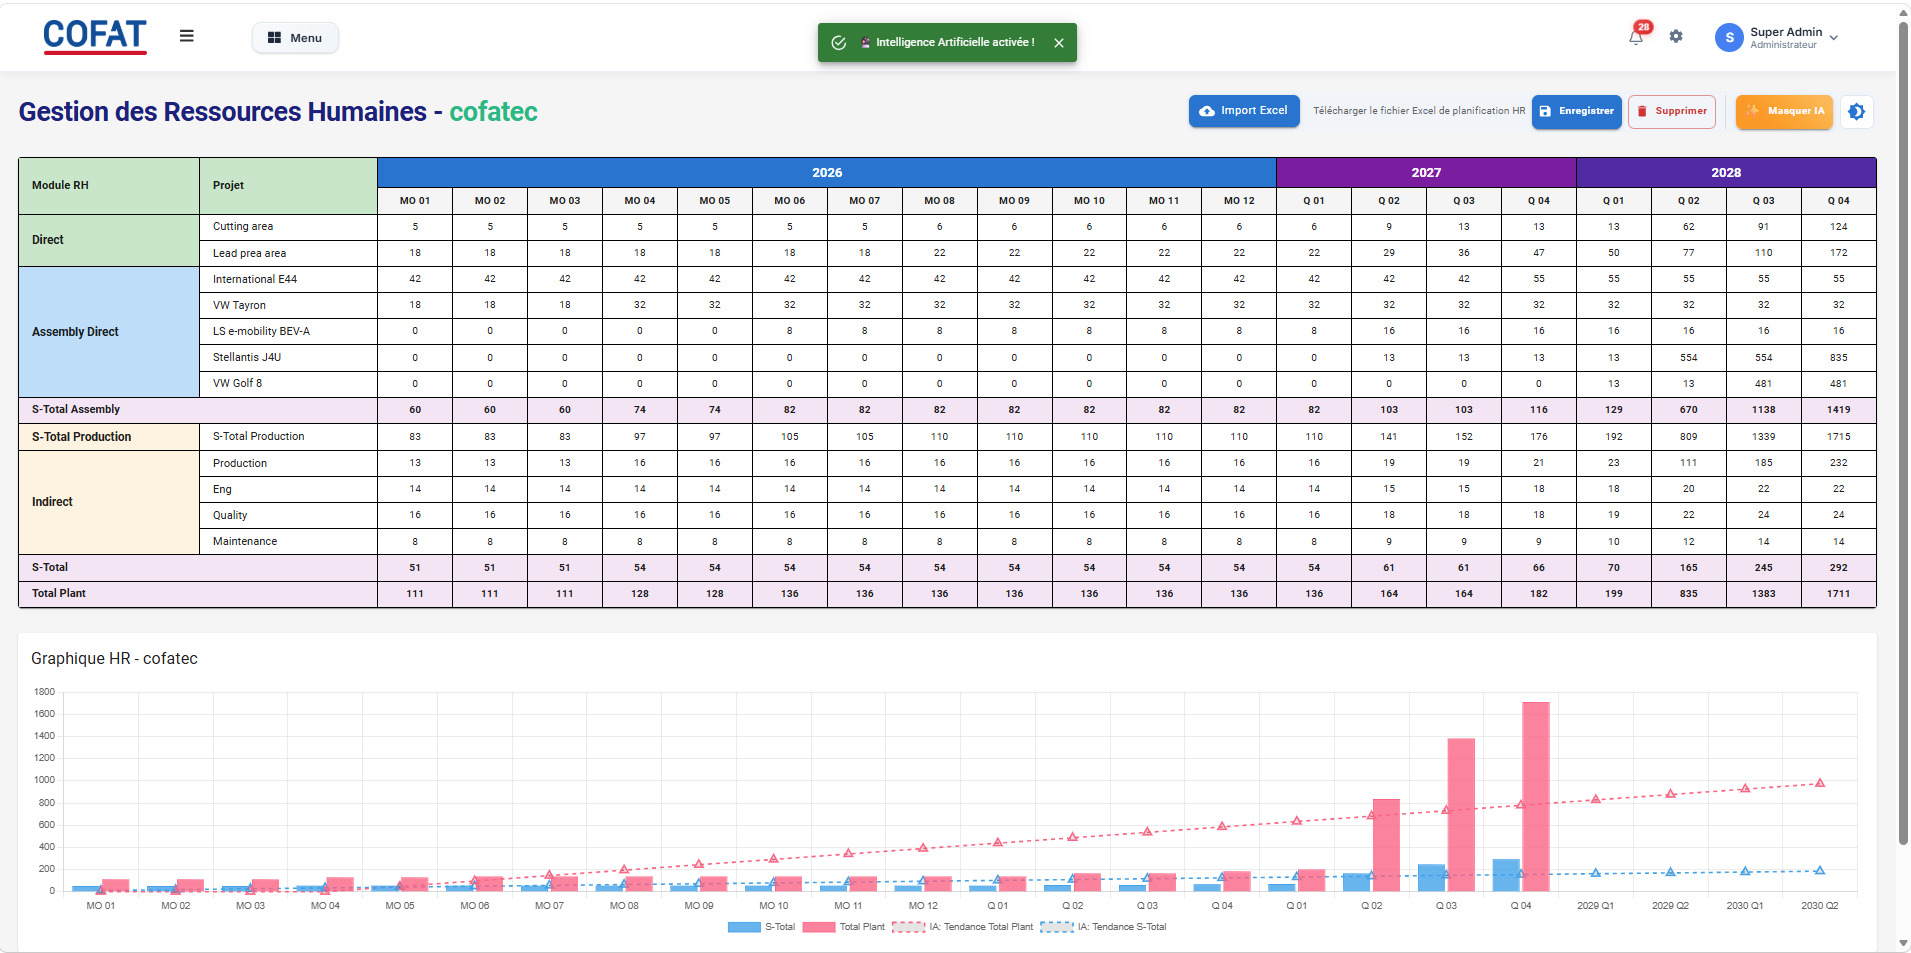
\includegraphics[width=1\textwidth]{img/gestion des resources humaines.png}
    \caption{Interface de planification temporelle des Ressources Humaines}
    \label{fig:planif_rh}
\end{figure}
\vspace{0.5cm}

\textbf{Analyse de la matrice temporelle RH (Figure \ref{fig:planif_rh}) :}
Ce module a été le plus complexe à modéliser ergonomiquement, car il présente une dimension temporelle très étendue. Le tableau, généré dynamiquement par un composant Ant Design, croise la dimension «~Métier~» avec la ligne de temps :
\begin{itemize}
    \item \textbf{Structuration en lignes} : Les effectifs sont regroupés par grandes catégories conformément au modèle \texttt{HR} réel : \textbf{Direct} (opérateurs machines), \textbf{Indirect} (qualité, maintenance, logistique, ingénierie) et \textbf{Assembly Direct} (opérateurs affectés à l'assemblage manuel des projets clients).
    \item \textbf{Structuration en colonnes (Time-Series)} : Pour offrir une vision de \textit{ramp-up} (montée en cadence), le système affiche la prévision mensuelle pour l'année courante (colonnes MO 01 à MO 12 pour 2025), puis bascule sur une granularité trimestrielle pour les années futures (colonnes Q01 à Q04 pour 2026 et 2027).
\end{itemize}

\textbf{Architecture du modèle \texttt{HR} :}
Le modèle Sequelize \texttt{HR} stocke chaque cellule du tableau comme une ligne indépendante, avec les champs \texttt{type} (nom de la ligne, ex: «~VW Tayron~»), \texttt{category} (Direct, Indirect, Assembly Direct, CALCULATION), \texttt{year}, \texttt{month} et \texttt{count} (effectif prévu). Cette structure normalisée, bien que plus volumineuse, permet d'additionner les effectifs par période avec une simple requête SQL d'agrégation, sans avoir à gérer des colonnes dynamiques côté backend.

\subsection{L'Ingénierie de l'Import Excel — Le Pipeline de données}
Saisir à la main des dizaines de cellules RH (12 mois + 8 trimestres par projet) dans un formulaire web aurait provoqué un rejet immédiat de l'application par les ingénieurs. C'est pourquoi un algorithme d'importation massive depuis des fichiers Excel (.xlsx) a été développé.

\textbf{Le processus technique détaillé en cinq étapes :}
\begin{enumerate}
    \item \textbf{Sélection côté React (Frontend)} : L'utilisateur clique sur le bouton «~Importer Excel~». Un élément \texttt{<input type="file">} s'ouvre. Le fichier sélectionné est inséré dans un objet \texttt{FormData} et envoyé au serveur via une requête \texttt{POST} Axios en \texttt{multipart/form-data}.
    \item \textbf{Réception via Multer (Middleware)}: À l'arrivée sur le port 9001, le middleware \texttt{multer} (configuré avec un \texttt{diskStorage}) intercepte le flux binaire. Il sauvegarde temporairement le fichier dans \texttt{/Uploads/budget/} avec un nom unique horodaté pour éviter les collisions, et filtre les extensions autorisées (\texttt{.xlsx}, \texttt{.xls}).
    \item \textbf{Parsing avec SheetJS (XLSX)} : Le contrôleur Node.js prend le relais. La bibliothèque \texttt{xlsx} ouvre le fichier depuis le chemin sauvegardé et convertit la première feuille du classeur en tableau d'objets JSON via \texttt{XLSX.utils.sheet\_to\_json()}.
    \item \textbf{Validation et nettoyage} : Le script parcourt le tableau JSON ligne par ligne. Il valide les types (un nombre attendu ne doit pas être du texte), rejette les lignes entièrement vides, et contrôle la présence des colonnes obligatoires. Les lignes invalides sont consignées dans un rapport d'erreur renvoyé au frontend, afin que l'ingénieur puisse corriger son fichier.
    \item \textbf{Insertion massive via Sequelize} : Si les données sont conformes, Sequelize exécute la méthode \texttt{bulkCreate()}, insérant les données en une seule transaction ACID optimisée. Le fichier temporaire est supprimé après traitement (\texttt{fs.unlinkSync()}), et le frontend affiche un message de réussite.
\end{enumerate}

\section{Sprint 3 : La Consolidation Mondiale (Cofat Group)}
Si la planification locale (Sprint 2) permet aux usines de respirer, c'est le module de Consolidation Groupe (Sprint 3) qui donne à la Direction (Admin) le véritable retour sur investissement du projet. Avant ce sprint, réunir les 10 entités de 6 pays différents prenait des jours de manipulation Excel. Désormais, le simple accès à l'onglet «~Cofat Group~» exécute des requêtes SQL d'agrégation massives qui produisent un état des lieux mondial en quelques secondes.

\subsection{Architecture de la consolidation — Le moteur d'agrégation}
La puissance de ce module repose sur la route \texttt{GET /api/cofat-group/consolidated} implémentée dans \texttt{routers/cofatGroupRoutes.js}. L'algorithme se déroule en trois phases :

\begin{enumerate}
    \item \textbf{Extraction} : Sequelize exécute un \texttt{EquipmentPlanning.findAll()} avec des \texttt{include} joints vers les modèles \texttt{Equipment} et \texttt{Site}. Cette requête SQL unique rapatrie l'ensemble des données de planification de tous les sites, avec les informations de contexte (nom de l'équipement, nom du site).
    \item \textbf{Agrégation JavaScript} : Les données sont regroupées en mémoire par \texttt{equipmentId} et par période (\texttt{year-month}) via un \texttt{reduce()}. Pour chaque groupe, les champs \texttt{machineNeed}, \texttt{availableMachine} et \texttt{toOrder} sont sommés. La charge globale (\texttt{load}) est accumulée en tant que ratio, puis multipliée par 100 pour le rendu en pourcentage.
    \item \textbf{Formatage et réponse} : Le résultat est transformé en un tableau JSON structuré, où chaque équipement expose la liste des sites qui le planifient et un objet \texttt{periods} contenant les métriques agrégées pour chaque mois/année.
\end{enumerate}

\subsection{Consolidation des Équipements}

\vspace{0.5cm}
\begin{figure}[H]
    \centering
    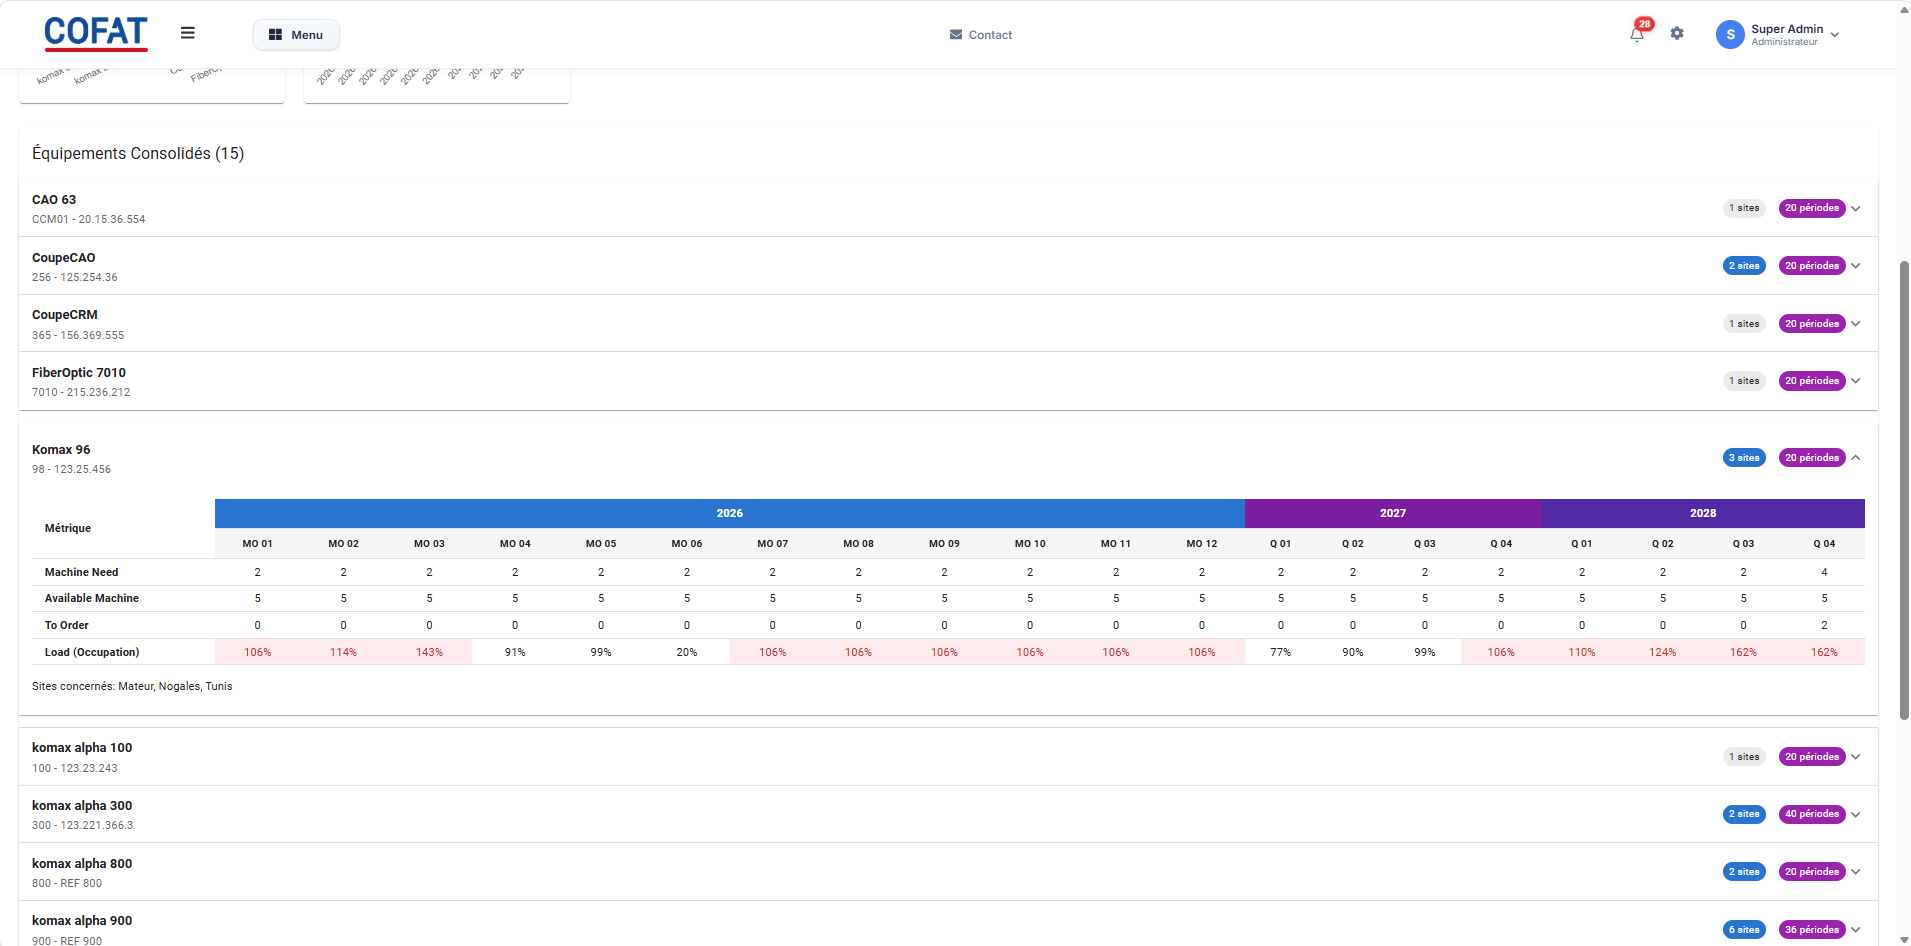
\includegraphics[width=0.9\textwidth]{img/consolidatinon cofatgroup Equipment.png}
    \caption{Tableau de consolidation mondiale des équipements industriels}
    \label{fig:conso_equipements}
\end{figure}
\vspace{0.5cm}

\textbf{Valeur métier de la consolidation (Figure \ref{fig:conso_equipements}) :}
L'impact stratégique est immédiat. Si l'usine du Mexique déclare un besoin urgent (\texttt{toOrder} = +2) sur une machine Komax, et que l'usine d'Égypte déclare un surplus sur ce même modèle (\texttt{toOrder} = -2), le tableau consolidé affichera un \textit{toOrder mondial} de zéro. La direction saura immédiatement qu'au lieu d'acheter deux machines neuves pour plusieurs centaines de milliers d'euros, elle doit simplement ordonner un transfert physique inter-sites. Ce type de décision, autrefois impossible sans semaines de travail manuel, est désormais visible en quelques clics.

\subsection{Consolidation des Espaces et des Ressources Humaines}
Le même principe d'agrégation est appliqué aux surfaces industrielles via la route \texttt{GET /api/cofat-group/space} et aux effectifs via \texttt{GET /api/cofat-group/hr}.

\vspace{0.5cm}
\begin{figure}[H]
    \centering
    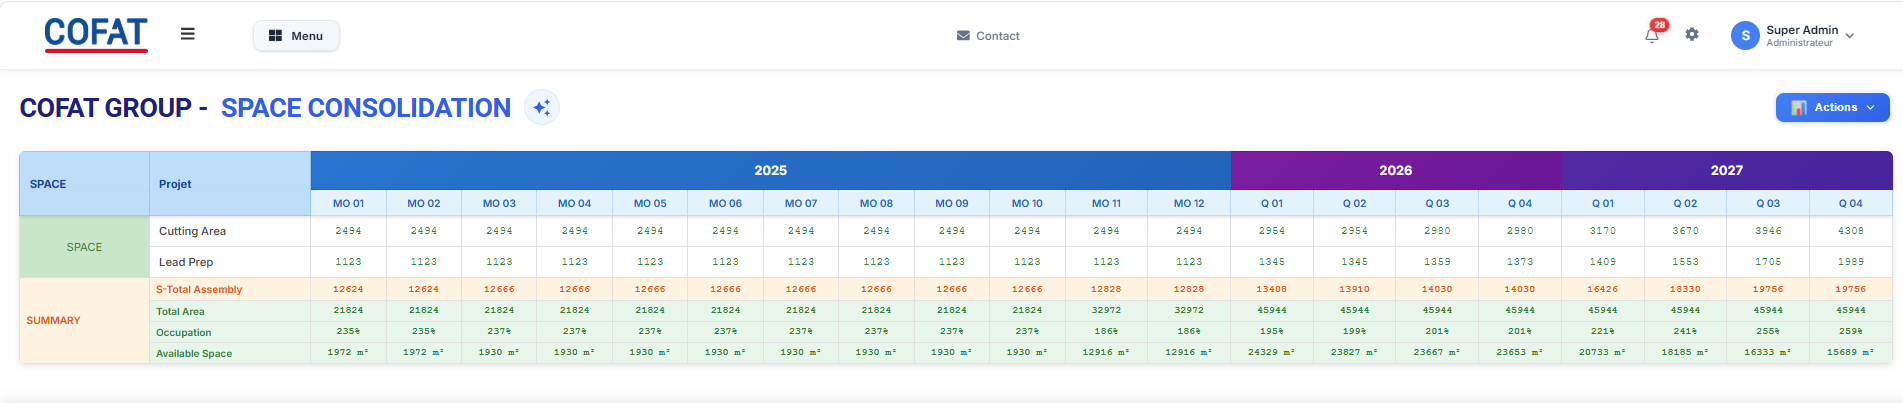
\includegraphics[width=0.9\textwidth]{img/cofat group space consolidation.png}
    \caption{Consolidation mondiale de l'occupation des usines COFAT}
    \label{fig:conso_espaces}
\end{figure}
\vspace{0.5cm}

\textbf{Algorithme de consolidation des espaces :}
L'algorithme d'agrégation des espaces est plus sophistiqué car il doit gérer des lignes de types différents (Cutting area, Lead prep, Assembly, Total Area). Le backend détecte dynamiquement les années et périodes disponibles en base, génère une liste ordonnée de mois, puis accumule les surfaces par type et par site. Les métriques globales (Total Area Needed, Available Space, Occupation Rate) sont calculées en priorité à partir des lignes explicites de la base (si un site a déclaré une ligne «~TOTAL AREA~»), avec un fallback calculé (somme des composants) si ces lignes sont absentes.

\vspace{0.5cm}
\begin{figure}[H]
    \centering
    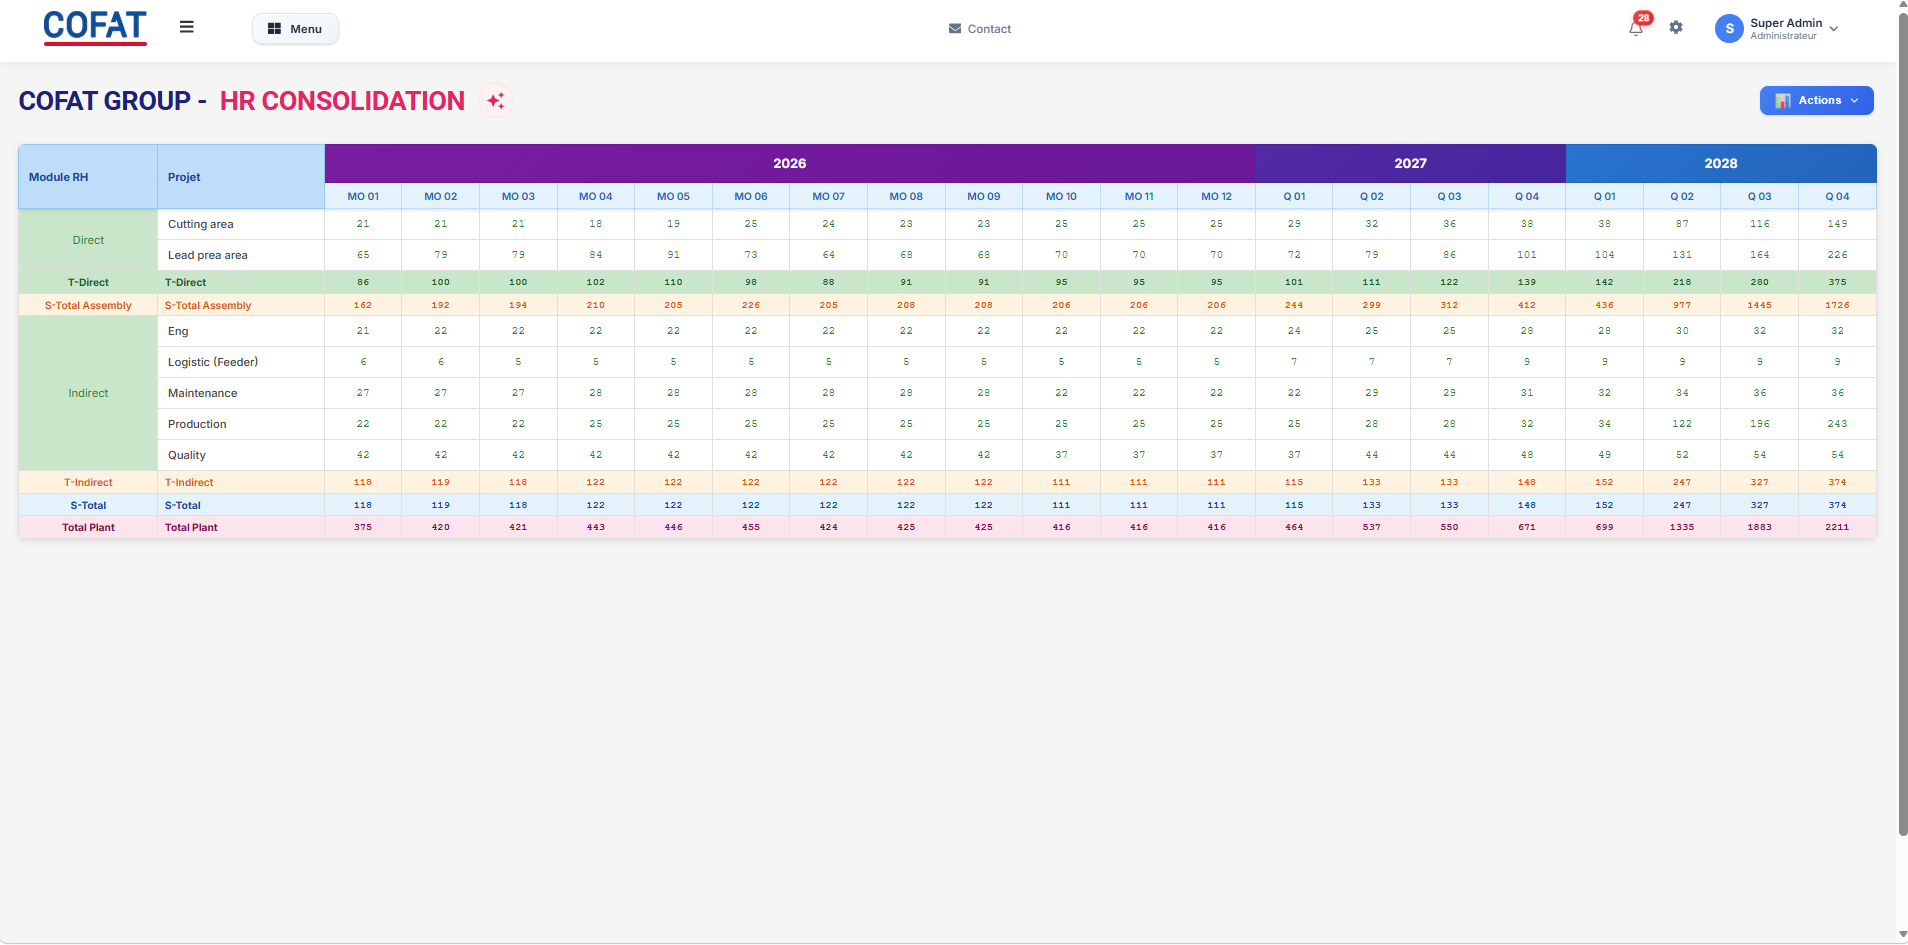
\includegraphics[width=1\textwidth]{img/cofat group HR consolidation.png}
    \caption{Tableau de consolidation RH mondial par projet et catégorie}
    \label{fig:conso_rh_table}
\end{figure}
\vspace{0.5cm}

\vspace{0.5cm}
\begin{figure}[H]
    \centering
    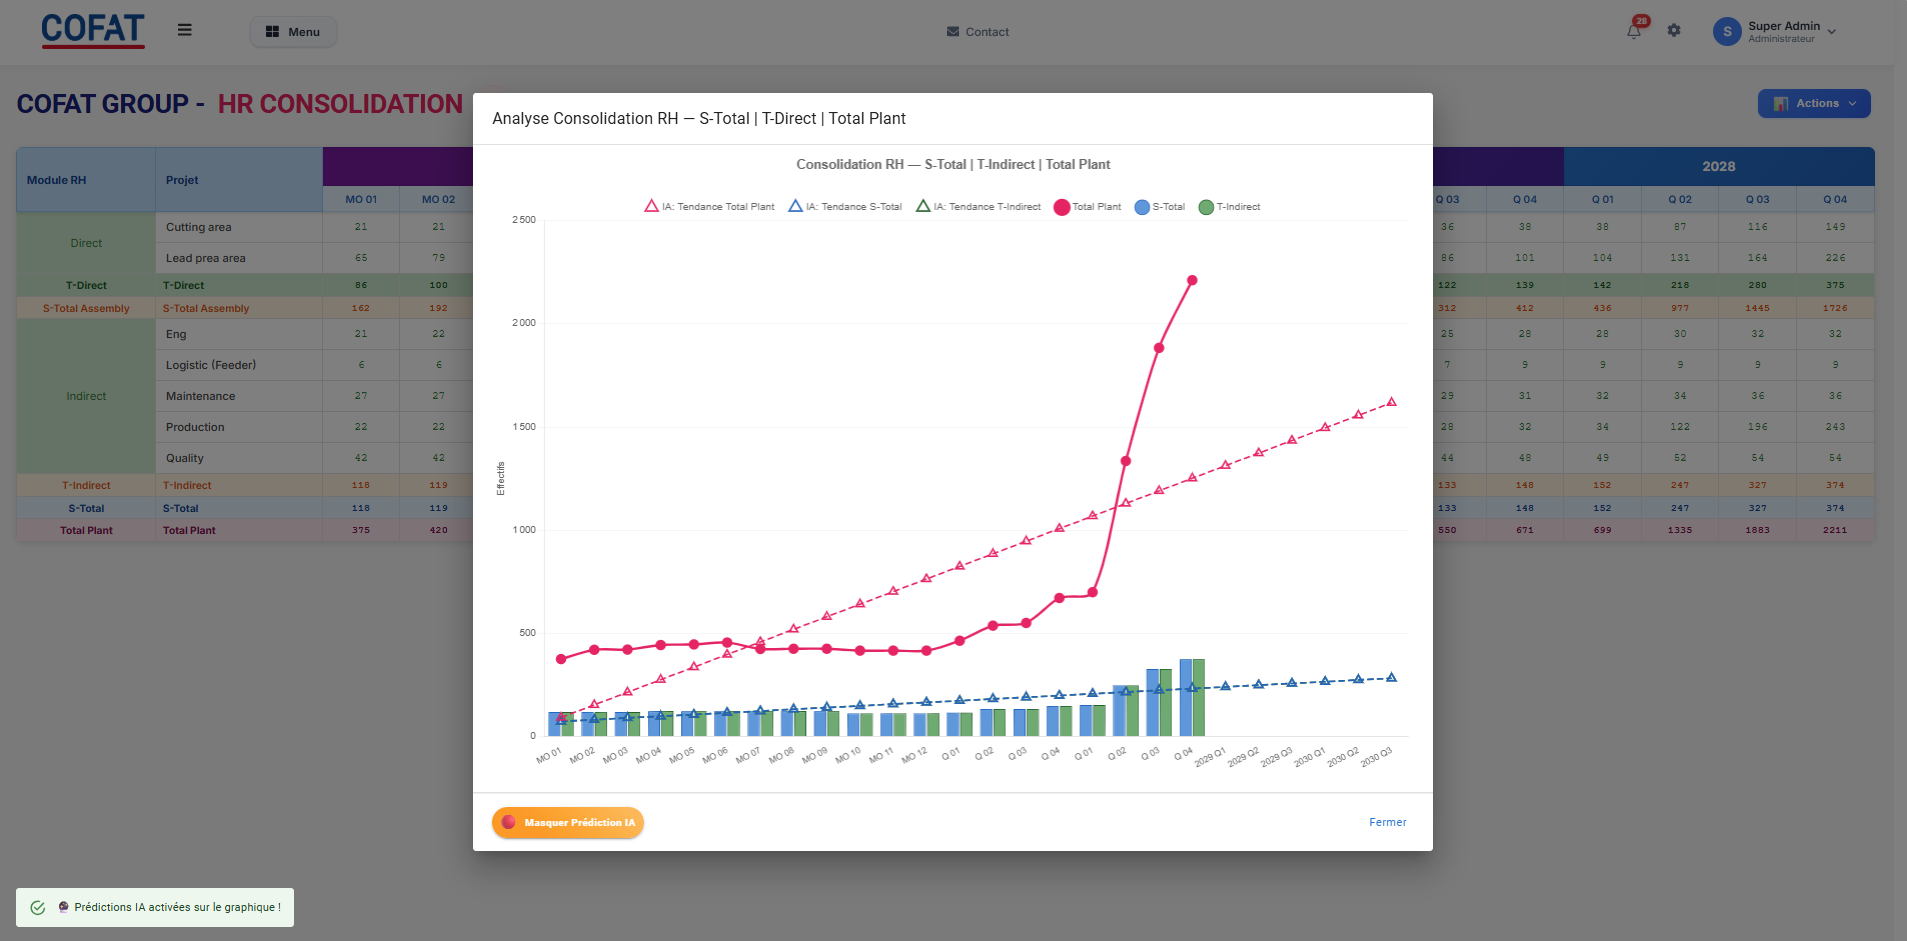
\includegraphics[width=0.9\textwidth]{img/analyse cofat group HR consolidation.png}
    \caption{Dashboard analytique de la montée en charge RH mondiale (Ramp-up)}
    \label{fig:conso_rh_graph}
\end{figure}
\vspace{0.5cm}

\textbf{Analyse de l'agrégation RH (Figures \ref{fig:conso_rh_table} et \ref{fig:conso_rh_graph}) :}
La Figure \ref{fig:conso_rh_table} affiche la somme matricielle des effectifs prévus pour les 10 sites sur 3 ans (2025-2027). L'algorithme de consolidation HR (\texttt{GET /api/cofat-group/hr}) regroupe les lignes par catégorie (Direct, Indirect, Assembly Direct) et par type de poste, en consolidant les noms de départements similaires via une normalisation (ex: «~Production~» et «~Production (Leader)~» sont fusionnés en une seule ligne «~Production~»).

Pour rendre ce mur de chiffres intelligible, l'application génère le Dashboard analytique de la Figure \ref{fig:conso_rh_graph} via \textit{Charts.js}. Ce graphique en barres empilées par période montre l'évolution de la main-d'œuvre nécessaire au fil des trimestres, offrant une vision lissée de la trajectoire de recrutement global.

\section{Le Catalogue : StandardInvestment V2}
Pour calculer les budgets nécessaires aux déficits capacitaires (\textit{toOrder}), il fallait uniformiser les bases de calcul entre les usines. Le Sprint 3 s'est clôturé par la réalisation du module \textit{StandardInvestment V2}, le dictionnaire mondial des prix d'équipements imposé par COFAT.

\vspace{0.5cm}
\begin{figure}[H]
    \centering
    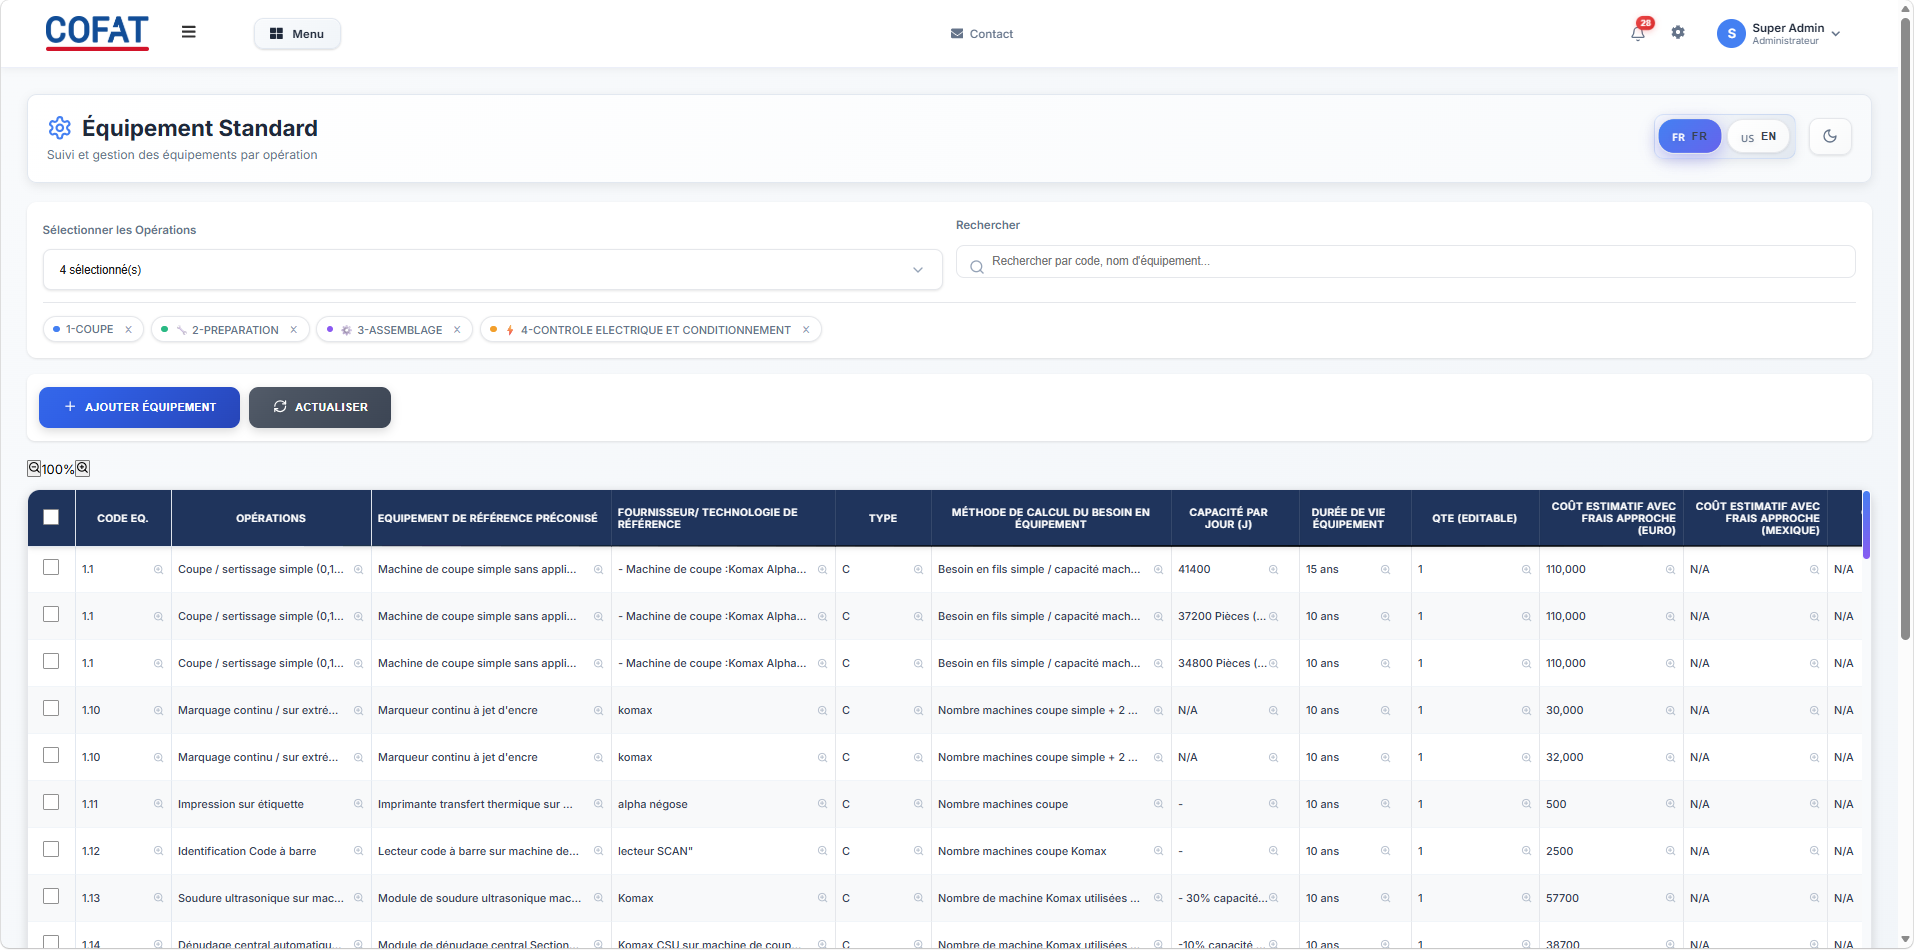
\includegraphics[width=0.9\textwidth]{img/equipement standard.png}
    \caption{Catalogue centralisé StandardInvestment V2}
    \label{fig:standard_equip}
\end{figure}
\vspace{0.5cm}

\textbf{Architecture technique du catalogue :}
Le modèle \texttt{StandardInvestmentV2} est défini directement dans le routeur \texttt{standardInvestmentV2Routes.js} (sans fichier modèle séparé) et s'appuie sur la table SQL \texttt{StandardInvestments\_V2}. Ses champs réels couvrent :
\begin{itemize}
    \item \textbf{\texttt{code\_eq}} : Le code identifiant unique de l'équipement (ex: 1.5, 2.23).
    \item \textbf{\texttt{operation\_prefix} (TINYINT)} : L'entier représentant la grande famille d'opération (1=COUPE, 2=PREPARATION, 3=ASSEMBLAGE, 4=CONTRÔLE, 5=TEST, 6=DIVERS). Cet index est utilisé pour un filtrage ultra-rapide en base.
    \item \textbf{\texttt{operation}, \texttt{equipment\_reference}, \texttt{supplier\_technology}} : Les informations descriptives de l'équipement.
    \item \textbf{\texttt{cost\_euro}, \texttt{cost\_mexican\_peso}, \texttt{cost\_brazil\_real}} : Les coûts estimatifs dans les trois devises géographiques du groupe.
    \item \textbf{\texttt{daily\_capacity}, \texttt{lifetime}} : Les paramètres techniques pour le calcul d'amortissement.
    \item \textbf{\texttt{is\_active} (BOOLEAN)} : Le catalogue utilise un \textbf{soft delete} — les équipements désactivés ne sont pas supprimés physiquement mais masqués (\texttt{is\_active = false}), préservant l'historique des décisions.
    \item \textbf{\texttt{version}} : La version du catalogue (actuellement \texttt{'v15'}), permettant de tracer les évolutions du référentiel dans le temps.
\end{itemize}

\textbf{Fonctionnalités de recherche avancée :}
La route \texttt{GET /api/standard-investments-v2} propose un filtre par famille d'opération (\texttt{?operationCodes=1,3}) utilisant l'index \texttt{operation\_prefix} pour des performances optimales, combiné à une recherche textuelle multi-champs (\texttt{?search=Komax}) via des clauses \texttt{LIKE} sur \texttt{code\_eq}, \texttt{operation}, \texttt{equipment\_reference} et \texttt{supplier\_technology}. Une pagination côté serveur (\texttt{?page=1\&limit=100}) évite de transférer le catalogue entier en une seule réponse.

\vspace{0.5cm}
\begin{figure}[H]
    \centering
    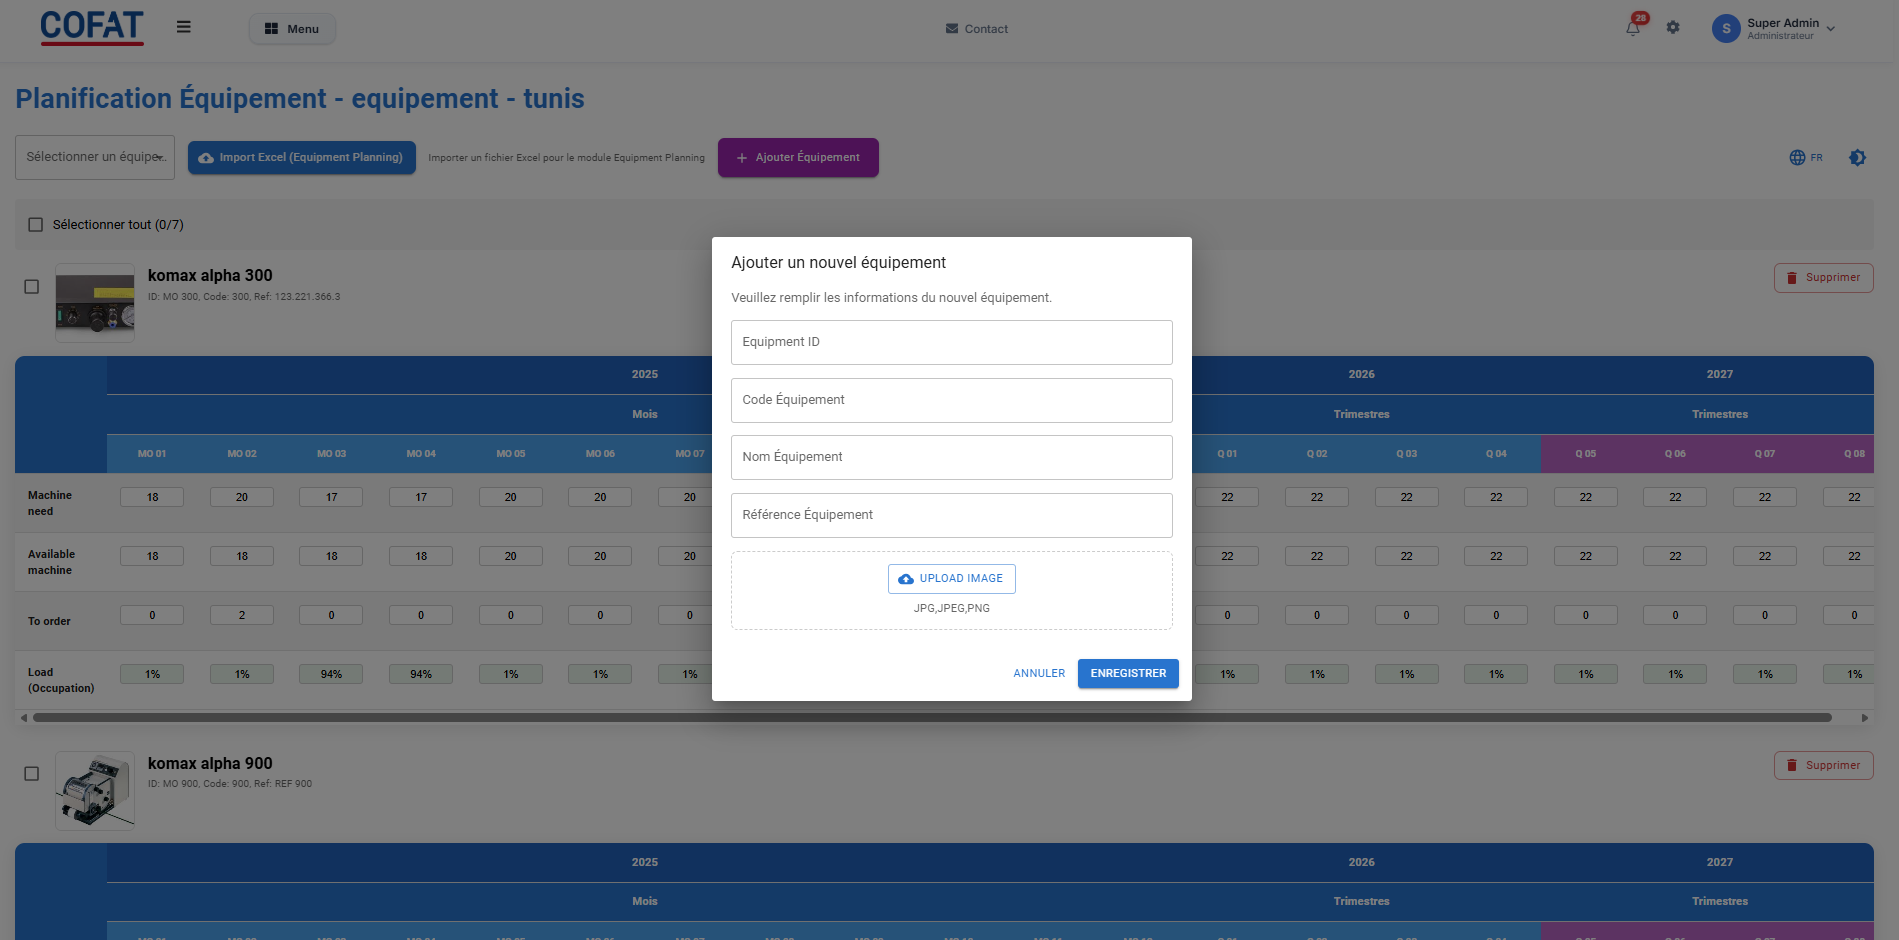
\includegraphics[width=0.8\textwidth]{img/equipement standard ajout 1.png}
    \caption{Formulaire d'ajout d'un équipement standard (Partie 1)}
    \label{fig:add_standard_1}
\end{figure}
\vspace{0.5cm}

\vspace{0.5cm}
\begin{figure}[H]
    \centering
    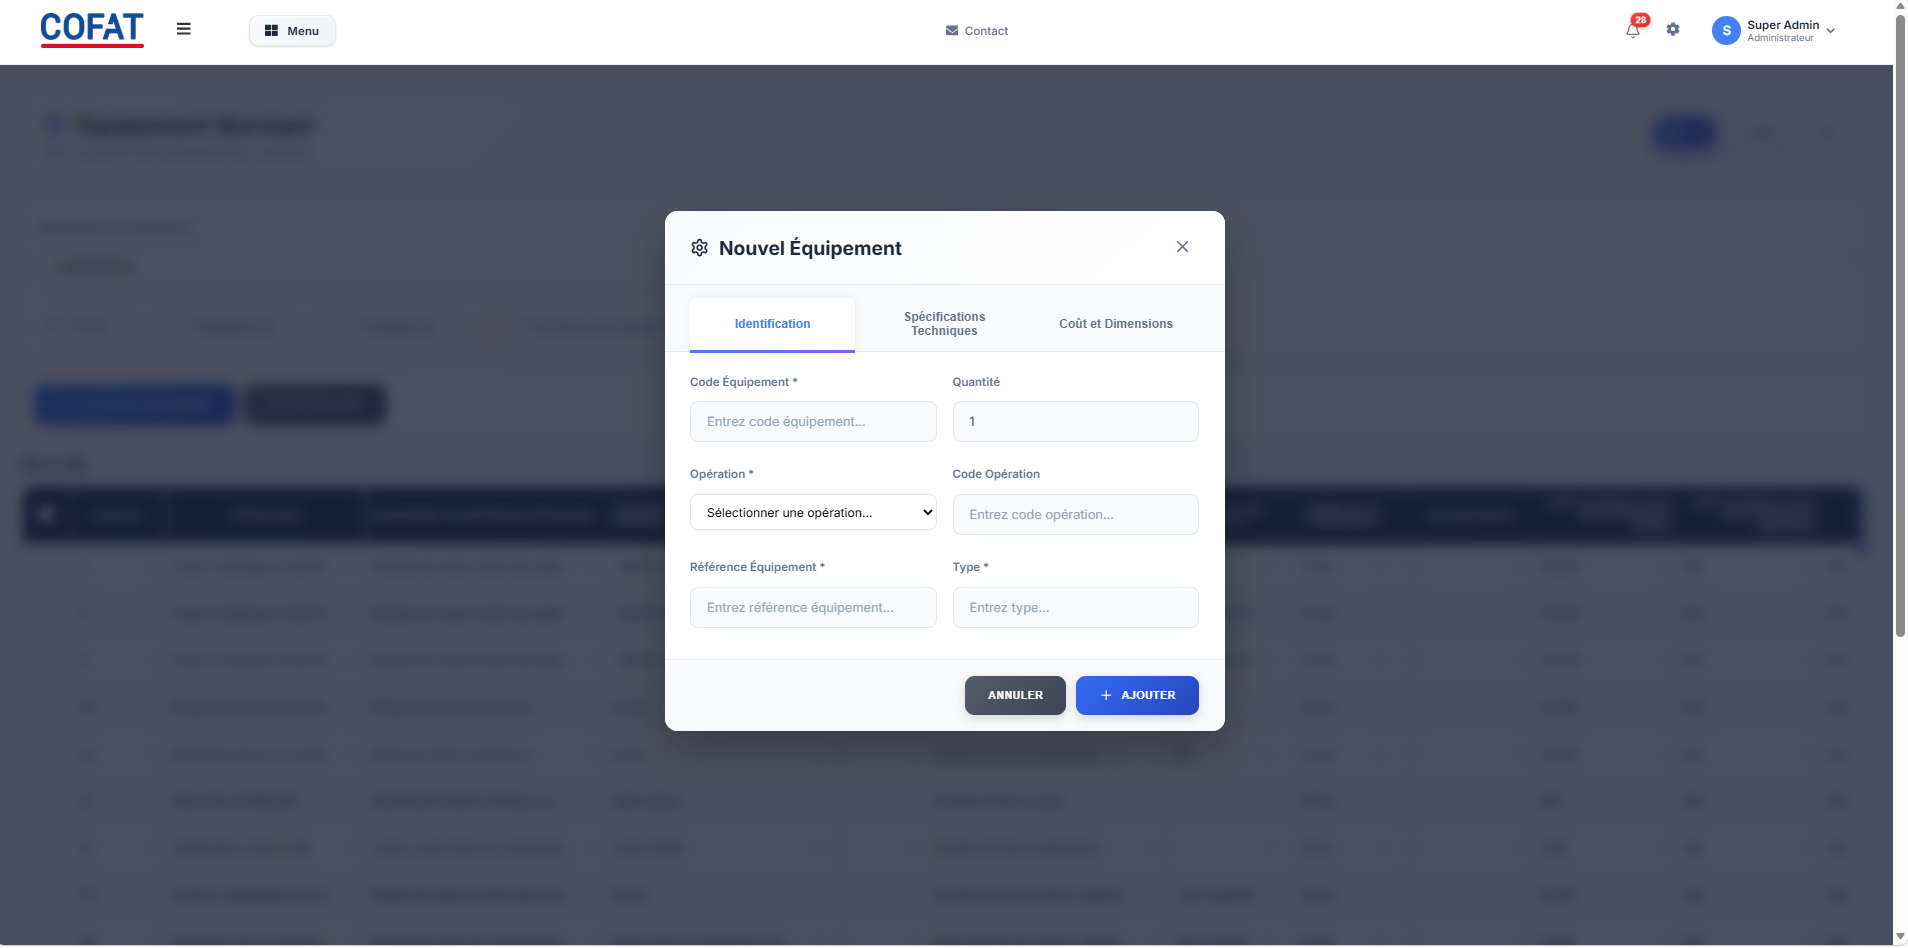
\includegraphics[width=0.8\textwidth]{img/equipement standard ajout 2.png}
    \caption{Formulaire d'ajout d'un équipement standard (Partie 2 : Coûts)}
    \label{fig:add_standard_2}
\end{figure}
\vspace{0.5cm}

\textbf{Gestion des Permissions : L'action de l'Acheteur (Achat) :}
Comme spécifié dans le Chapitre 2, la création (Figures \ref{fig:add_standard_1} et \ref{fig:add_standard_2}) ou la désactivation de standards est réservée à l'Administrateur central. L'Acheteur, en tant que négociateur externe, possède des droits précis sur ce catalogue : sa seule action est de mettre à jour les montants dans les colonnes des coûts estimatifs (\texttt{cost\_euro}, \texttt{cost\_mexican\_peso}, \texttt{cost\_brazil\_real}) suite à ses négociations fournisseurs. Ces prix mis à jour sont utilisés par le système pour monétiser la colonne \textit{toOrder} des planifications locales.

\vspace{0.5cm}
\begin{figure}[H]
    \centering
    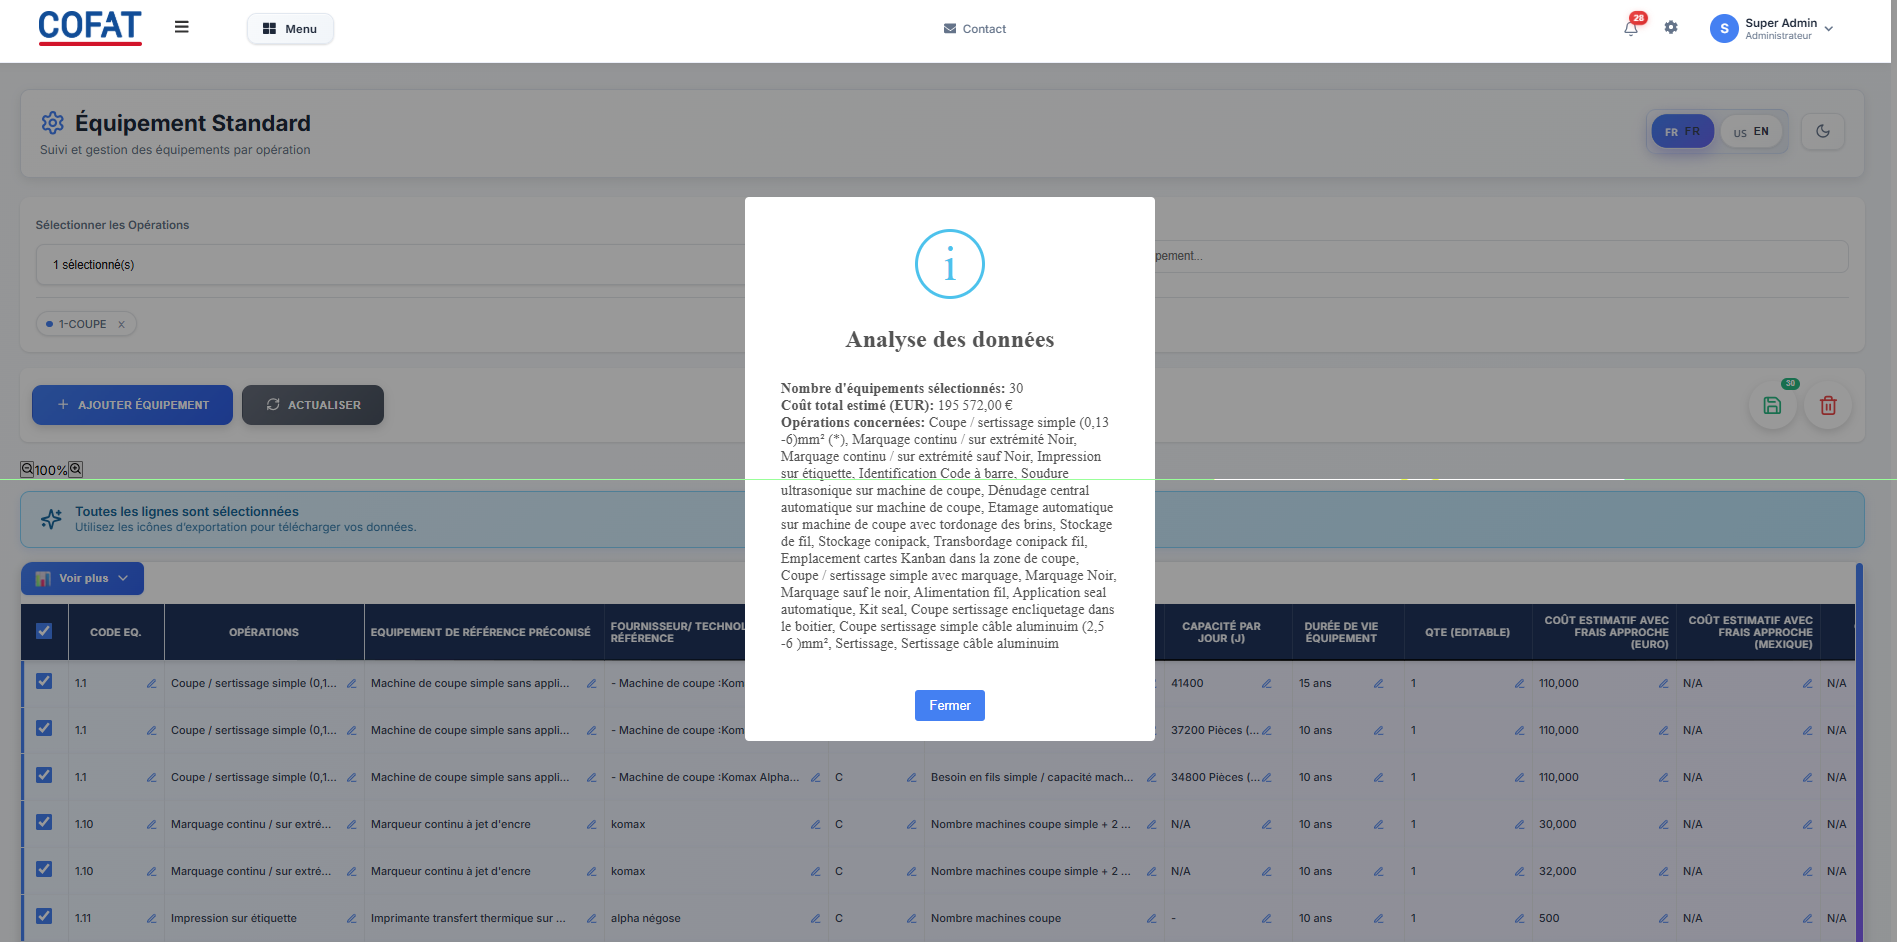
\includegraphics[width=0.9\textwidth]{img/analyse equipement standard.png}
    \caption{Analyse graphique du catalogue des équipements standards}
    \label{fig:analyse_standard}
\end{figure}
\vspace{0.5cm}

\section{Conclusion}
Les Sprints 2 et 3 ont transformé une vision théorique en un outil industriel redoutable. Le déploiement des interfaces de planification locale offre aux responsables d'usine l'autonomie et la clarté nécessaires à la gestion de leurs capacités. Le pipeline d'import Excel — de Multer au \texttt{bulkCreate} Sequelize, en passant par la validation des données — garantit une transition numérique sans friction pour les employés habitués aux tableurs.

En capitalisant sur cette base de données fraîchement alimentée, le moteur de consolidation mondiale (Sprint 3) délivre en quelques secondes des tableaux de bord interactifs à la direction. Le catalogue \textit{StandardInvestment V2}, avec son système de soft delete, sa recherche multi-critères et ses coûts multi-devises, offre à l'Achat le référentiel centralisé indispensable pour standardiser l'évaluation financière des investissements industriels à l'échelle mondiale.

L'étape ultime du projet, couverte par le Sprint 4 (Chapitre 5), consistera à numériser le circuit de gestion financière des investissements non-industriels à travers un workflow collaboratif entre les Site Managers et le département des Achats.